\documentclass[twoside,11pt]{article}
\usepackage[T1]{fontenc}
\usepackage{blindtext}
\usepackage{siunitx}
\sisetup{output-exponent-marker=\ensuremath{\mathrm{e}}}

% Any additional packages needed should be included after jmlr2e.
% Note that jmlr2e.sty includes epsfig, amssymb, natbib and graphicx,
% and defines many common macros, such as 'proof' and 'example'.
%
% It also sets the bibliographystyle to plainnat; for more information on
% natbib citation styles, see the natbib documentation, a copy of which
% is archived at http://www.jmlr.org/format/natbib.pdf

% Available options for package jmlr2e are:
%
%   - abbrvbib : use abbrvnat for the bibliography style
%   - nohyperref : do not load the hyperref package
%   - preprint : remove JMLR specific information from the template,
%         useful for example for posting to preprint servers.
%
% Example of using the package with custom options:
%
% \usepackage[abbrvbib, preprint]{jmlr2e}

\usepackage[preprint]{jmlr2e}

% Definitions of handy macros can go here

\newcommand{\dataset}{{\cal D}}
\newcommand{\fracpartial}[2]{\frac{\partial #1}{\partial  #2}}

% ================ START OF NON-TEMPLATE SETUP ================ %
\usepackage[dvipsnames]{xcolor}
\usepackage{amsmath,amssymb}
\usepackage{xfrac}

% Silence unneeded warnings.
\usepackage{silence}
\WarningFilter{caption}{Unknown document class}

% For drawing automata.
\usepackage{tikz}
\usetikzlibrary{arrows.meta,matrix,automata,shapes,positioning}
\tikzstyle{elbl} = [fill=white,inner sep=1pt,font=\footnotesize,>=stealth]

% For tables.
\usepackage{booktabs,multirow}
\usepackage{subcaption}
\usepackage[font=small,labelfont=bf]{caption}

% Useful shorthand.
\newcommand{\tsc}[1]{\textsc{#1}}
\newcommand{\ttt}[1]{\texttt{#1}}
\newcommand{\tbf}[1]{\textbf{#1}}

% Shorthand for MLRegTest factors.
\newcommand{\tttx}[1]{\ttt{#1}\xspace}
\newcommand{\Alpha}{\tttx{Alph}}
\newcommand{\Tier}{\tttx{Tier}}
\newcommand{\Class}{\tttx{Class}}
\newcommand{\kay}{\tttx{k}}
\newcommand{\jay}{\tttx{j}}
\newcommand{\eye}{\tttx{i}}
\newcommand{\TrainSize}{\tttx{TrainSize}}
\newcommand{\TestType}{\tttx{TestType}}
\newcommand{\NNType}{\tttx{NNType}}
\newcommand{\AlgoType}{\tttx{AlgoType}}

% Code repository url
\newcommand{\repo}{https://github.com/adil-soubki/mlrt}

% Use these to change spacing of lists.
\usepackage{enumitem}
\setlist[enumerate]{
    topsep=0pt,itemsep=-0.5ex,
    partopsep=0.5ex,parsep=0.5ex
}
\setlist[itemize]{
    topsep=0pt,itemsep=-0.5ex,
    partopsep=0.5ex,parsep=0.5ex,
    leftmargin=10pt
}

% Set the paper title here.
\newcommand{\papertitle}{Short Strings Matter More for State Merging Algorithms than They Do for Neural Learning Systems}


\newcommand{\todo}[1]{\textcolor{red}{(TODO: {#1})}}
\newcommand{\sarah}[1]{\textcolor{cyan}{(SP: {#1})}}
\newcommand{\logan}[1]{\textcolor{orange}{(LS: {#1})}}


% ================= END OF NON-TEMPLATE SETUP ================= %


% Heading arguments are {volume}{year}{pages}{date submitted}{date published}{paper id}{author-full-names}

\usepackage{lastpage}
\jmlrheading{23}{2022}{1-\pageref{LastPage}}{1/21; Revised 5/22}{9/22}{21-0000}{}

% Short headings should be running head and authors last names

\ShortHeadings{Short Strings Matter More for State Merging}{}
\firstpageno{1}

\begin{document}

\title{\papertitle}

\author{\name{~Anonymous~Review~Copy}}
% \author{
%     \name Logan Swanson
%     \email logan.swanson@stonybrook.edu\\
%     \addr Department of Lingustics \\
%     Institute for Advanced Computational Science \\
%     Stony Brook University
%     \AND
%     \name Sarah Payne
%     \email sarah.payne@stonybrook.edu\\
%     \addr Department of Linguistics \\
%     Institute for Advanced Computational Science \\
%     Stony Brook University
%     \AND
%     \name Adil Soubki
%     \email asoubki@cs.stonybrook.edu\\
%     \addr Department of Computer Science \\
%     Institute for Advanced Computational Science \\
%     Stony Brook University
%     \AND
%     \name Sam van der Poel
%     \email samvanderpoel@gatech.edu\\
%     \addr Department of Computer Science \\
%     Georgia Tech University \\
%     \AND
%     \name Jeffrey Heinz
%     \email jeffrey.heinz@stonybrook.edu\\
%     \addr Department of Linguistics \\
%     Institute for Advanced Computational Science \\
%     Stony Brook University
% }

\editor{}

\maketitle


% trailing '%' for backward compatibility of .sty file
\begin{abstract}%
  MLRegTest \citep{mlregtest} is a benchmark for learning regular
  languages from positive and negative data.
  \citet{adil23} examine the performance of the
  state-merging algorithms RPNI, EDSM, and ALERGIA on a preliminary
  version of MLRegTest and found that the neural learning models
  generally outperformed the state-merging algorithms on this
  benchmark.  However, since MLRegtTest excludes strings less than
  length 19 in order to achieve a balance of positive and negative
  strings in training, development and test sets across all languages
  in the benchmark, \citet{adil23} also report
  follow-up experiments which included shorter training strings and
  shows they dramatically improve the performance of the state-merging
  algorithms. They did not examine the performance of the neural
  models with shorter strings.
  
  In this context, this paper makes the following
  contributions. First, it utilizes the final version of MLRegTest,
  not the preliminary version.  Second, instead of running RPNI and
  EDSM, it conductas a limited gridsearch over the parameters provided
  by the flexfringe software \citep{flexfringe-short, flexfringe} to
  find suitable hyperparameters for merging states. Third, it reports
  the results of this state-merging algorithm on five experimental
  setups: only-short strings, the small data plus short strings, the
  small data without short strings, the medium data plus short
  strings, the medium data without short strings. Fourth, it subjects
  the neural baselines from \citet{mlregtest} to these same
  experiments for comparison.

  We conclude that the neural systems, especially the gated recurrent
  unit, generally outperforms the state-merging algorithm across the
  benchmarks, with some interesting caveats. The state-merging
  algorithm outperforms the neural methods on regular languages that
  count modulo some positive integer. Secondly, the state-merging
  algorithms do much better when short strings are included, while the
  neural learning systems only see moderate improvement.
  

\end{abstract}

\begin{keywords}
  state-merging, regular languages, finite-state automata, neural networks
\end{keywords}


\section{Introduction}

\todo{Currently identical to abstract. Change abstract?}

  MLRegTest \citep{mlregtest} is a benchmark for learning regular
  languages from positive and negative data.
  \citet{adil23} examine the performance of the
  state-merging algorithms RPNI, EDSM, and ALERGIA on a preliminary
  version of MLRegTest and found that the neural learning models
  generally outperformed the state-merging algorithms on this
  benchmark.  However, since MLRegtTest excludes strings less than
  length 19 in order to achieve a balance of positive and negative
  strings in training, development and test sets across all languages
  in the benchmark, \citet{adil23} also report
  follow-up experiments which included shorter training strings and
  shows they dramatically improve the performance of the state-merging
  algorithms. They did not examine the performance of the neural
  models with shorter strings.
  
  In this context, this paper makes the following
  contributions. First, it utilizes the final version of MLRegTest,
  not the preliminary version.  Second, instead of running RPNI and
  EDSM, it conductas a limited gridsearch over the parameters provided
  by the flexfringe software \citep{flexfringe-short, flexfringe} to
  find suitable hyperparameters for merging states. Third, it reports
  the results of this state-merging algorithm on five experimental
  setups: only-short strings, the small data plus short strings, the
  small data without short strings, the medium data plus short
  strings, the medium data without short strings. Fourth, it subjects
  the neural baselines from \citet{mlregtest} to these same
  experiments for comparison.

  We conclude that the gated recurrent unit outperforms the
  all state-merging algorithm in richer data regimes, with some interesting
  caveats. The state-merging algorithm outperforms the neural methods
  on regular languages that count modulo some positive
  integer. Secondly, the state-merging algorithms do much better when
  short strings are included, while the neural learning systems only
  see moderate improvement.
  
\section{Learning Systems} \label{sec:bg}


\subsection{State-Merging Systems}\label{sec:ff}

Following \citet{adil23}, we use the state-merging software
\textsc{FlexFringe} \citep{flexfringe},\footnote{We use the same
  version of \textsc{FlexFringe} used by \citeauthor{adil23}: commit
  \texttt{4d1449c} of the software available
  \href{https://github.com/tudelft-cda-lab/FlexFringe/commit/4d1449c4d0cfb3fc5f9a954d5c3a24a11a593a5c\#diff-67290ef9e84d355c83cbd9a0bda3be39e2e14836990458cfcc070506a7e448c2}{here}.
} which implements a range of state-merging strategies using the
red/blue framework (see \citet{Higuera2010}). For instance, the
algorithms EDSM \citep{edsm} and RPNI \citep{rpni} are particular
strategies which \textsc{FlexFringe} can instantiate.  Generally
speaking, these algorithms construct a prefix tree from their input
and search for pairs of states to merge.

In general, \textsc{FlexFringe} scores pairs of states for their
``mergability'' and merges states with sufficient scores in some
order, as determined by various parameter
settings. \textsc{FlexFringe} also can also learn stochastic regular
languages with state-merging algorithms such as ALERGIA
\citep{CarrascoOncina1994, carr99}. However, we exclude ALERGIA from
consideration because of its comparatively low performance noted by
\citeauthor{adil23}.

\textsc{FlexFringe} provides several parameters which determine its
state-merging strategy.  To find the best model, we conducted a
limited gridsearch over the following subset: \texttt{PerformFirst}
(EDSM vs. RPNI), \texttt{Extend} (color blue states red that cannot be
merged with any red), \texttt{ShallowFirst} (consider coloring blue
states closest to the root first), and \texttt{SearchStrategy}
(searchdeep, searchlocal, searchglobal, searchpartial, or none).  Grid
searching was done on the small partition of the \textsc{PlusShort}
data using overall accuracy on the \textsc{Small} development set
(these data sets are described in \S\ref{sec:eval}). The best
performing model, used in the remainder of the paper, was
\texttt{PerformFirst = 0} (i.e., RPNI), \texttt{Extend = 1},
\texttt{ShallowFirst = 0}, and \texttt{SearchStrategy = SearchDeep}.

The SearchDeep strategy deserves some discussion. This strategy
considers the tree of all possible sequences of merges and the sizes
of the resulting DFA. It ultimately returns the DFA with the fewest
number of states. Given that the tree representing all possible
sequences of merges is quite large (and grows larger with the size of
the initial prefix tree), it is time-consuming to run.

We held several other parameters at their default state because
modifying them led to errors in the \texttt{FlexFringe}
executable. These are: \texttt{ReverseTraces}, \texttt{DepthCheck},
\texttt{SymbolCheck}, \texttt{SinksOn}, \texttt{SinkCount}, and
\texttt{MergeScore}. However, we have since learned more about these
parameters (Sicco Verweer, p.c.), and we believe we can avoid these
errors in the future. We plan to run a more comprehensive grid search
this summer.

\subsection{Neural Systems}
Following \citet{mlregtest}, we test four neural architectures, all
consisting of a trainable embedding layer followed by a unidirectional
recurrent module (either a \textbf{\textsc{Simple}} RNN, a
\textbf{GRU}, or an \textbf{LSTM}) or two consecutive
\textbf{\textsc{Transformer}} blocks, dense feed-forward layers,
dropout, layer normalization, and softmax activation.  All NNs use the
same hyperparameters as \citeauthor{mlregtest}.\footnote{The
  implementations of the neural networks are available at
  \href{https://github.com/heinz-jeffrey/subregular-learning/}{https://github.com/heinz-jeffrey/subregular-learning/}}

\section{Experimental Setup}\label{sec:eval}

\textsc{MLRegTest} \citep{mlregtest} contains training, development,
and test data from 1,800 regular languages. The languages were
organized along three dimensions: alphabet size (4, 16, 64), logical
complexity (monadic second order, first order, propositional,
conjunctions of negative literals, disjunctions of positive literals),
and ordering relation (successor, precedence, tier-successor).

The datasets for each language come in three sizes: \textsc{Small}
(1,000 strings), \textsc{Medium} (10,000 strings), and \textsc{Large}
(100,000 strings). For each language, the datasets are nested;
\textsc{Small} is contained in \textsc{Medium}, which is contained in
\textsc{Large}. Each dataset includes equal numbers of positive and
negative strings.

The training sets contain strings of lengths 20-29, sampled with
replacement. The development sets also contain strings of lengths
20-29, sampled without replacement in a manner to keep the development
sets disjoint from the training set.

\textsc{MLRegTest} contains four test sets per language, based on the
string length and the method of generation. \textsc{Short} sets have
strings of length 20-29, and \textsc{Long} sets have strings of length
31-50. \textsc{Random} test sets were created by sampling without
replacement in a manner to keep the development sets disjoint from the
training and development sets. \textsc{Adversarial} sets sampled pairs
of positive and negative examples with an edit distance of 1 in a
manner to keep the development sets disjoint from the training and
development sets. (Of course for the \textsc{Long} test sets nothing
needed to be done to ensure they were disjoint from the training and
development sets.)

Following \citet{mlregtest} and \citet{adil23}, we evaluate trained
models only on the \textsc{Large} test sets. Henceforth, we refer to
these test sets as SR, LR, SA, LA for \textsc{Short Random, Long
  Random, Short Adversarial}, and \textsc{Long Adversarial},
respectively.

As mentioned, the training strings in \textsc{MLRegTest} are of length
20-29.  \citeauthor{adil23} found that augmenting the training set
with up to 1,000 positive and negative strings of length 1-19
significantly improved \textsc{FlexFringe} performance despite
sacrificing the balance of positive and negative examples.

\citeauthor{adil23} built a short training set for each language as
follows. For each length, 25 positive and 25 negative strings were
sampled with replacement.  If no positive negative strings of a given
length existed, none were drawn for that length.

In this work, we rebuilt the short training sets using that same
recipe because \citeauthor{adil23} used a preliminary version, and we
used the published version.\footnote{MLRegTest is publicly available
  with Dryad \url{https://doi.org/10.5061/dryad.dncjsxm4h} under the
  license \emph{CC0 1.0 Universal (CC0 1.0) Public Domain Dedication}
  (\url{https://creativecommons.org/publicdomain/zero/1.0/}).}

We conducted three kinds of experiments. In the \textsc{OnlyShort}
experiments, only the short training set was used for training. In the
\textsc{PlusShort} experiments, the training set was made up of the
original \textsc{MLRegTest} training sets augmented with the short
training set. In the \textsc{OnlyLong} experiments, the original
\textsc{MLRegTest} training sets were used (without the short training
set).

We excluded languages with alphabet sizes of 64, thus considering
1,140, in order to compare our results with \citet{adil23}. This
submission also excludes the Large training sets because the
SearchDeep strategy caused \textsc{FlexFringe} to run too long during
training.

Thus for each language, for each learning system, we considered five
training regimes: \textsc{Only Short, Small Plus Short, Medium Plus
  Short, Only Small, Only Medium}. Each trained model was tested on
the aforementioned four test sets.\footnote{Note that the
  \textsc{Short} test sets contain strings of length 20-29, while the
  Short training sets contain strings of length 1-19. We apologize for
  any confusion.}

The \textsc{PlusShort} and \textsc{OnlyLong} experiments essentially
replicate the experiments in \citet{adil23} on a preliminary version
of MLRegTest. The \textsc{OnlyShort} experiments are novel to this
paper and help clarify the role short training strings play for
learning regular languages.

\section{Results} \label{sec:results}

% FF
%   Mid_OL    Mid_PS  Small_OL  Small_OS  Small_PS 
% 0.5886030 0.7991419 0.5465408 0.7374390 0.7750243 

% Simple
%    Mid_OL    Mid_PS  Small_OL  Small_OS  Small_PS 
% 0.7650535 0.7761876 0.7037516 0.6649203 0.7224823 

% GRU
% Mid_OL    Mid_PS  Small_OL  Small_OS  Small_PS 
% 0.9165559 0.9531099 0.8329323 0.7941359 0.9094917 

% LSTM
%  Mid_OL    Mid_PS  Small_OL  Small_OS  Small_PS 
% 0.8234046 0.8692251 0.6054237 0.6336763 0.7201030 

% Transformer
%   Mid_OL    Mid_PS  Small_OL  Small_OS  Small_PS 
%   0.8010169 0.8136149 0.7488404 0.6965861 0.7623821

\subsection{Overall performance}

Table \ref{tab:overall-scores} gives the mean F1 score of each model
across languages, experiments, and test sets. Importantly, the results
in the \textsc{PlusShort} and \textsc{OnlyLong} experiments are
consistent with \citet{adil23} and \citet{mlregtest}, respectively.

\begin{table}[t!]
\centering
\begin{tabular}{rccccccc}
  \toprule
                 & \textsc{Only } & \textsc{Small}      & \textsc{Medium}     & \textsc{Only}  & \textsc{Only}   \\
  \textsc{Model} & \textsc{Short} & \textsc{Plus Short} & \textsc{Plus Short} & \textsc{Small} & \textsc{Medium} \\
  \midrule
  FlexFringe     & .737           & .775                & .799                & .547           & .589            \\
  Simple         & .665           & .722                & .776                & .704           & .765            \\
  LSTM           & .634           & .720                & .869                & .605           & .823            \\
  Transformer    & .697           & .762                & .814                & .749           & .801            \\
  GRU            & \textbf{.794}  & \textbf{.909}       & \textbf{.953}       & \textbf{.833}  & \textbf{.917}   \\
  \bottomrule
\end{tabular}
\caption{Mean F1 score across all test sets for all languages by
  experiment type and model.}
\label{tab:overall-scores}
\end{table}

The GRU consistently outperforms the other models across all
experiments. Interestingly however, \textsc{FlexFringe} outperforms
the other NNs in the \textsc{OnlyShort} and \textsc{PLusShort}
experiments. In all other training conditions, the NNs outperform
\textsc{FlexFringe}, with the exception of the Simple RNN in the
\textsc{Medium Plus Short} condition.

Another important observation is that without the Short training data
(e.g. comparing \textsc{Small Plus Short} with \textsc{Only Small}),
\textsc{FlexFringe}'s performance drops at least 20 points. On the
other hand, the NNs, across the board, are much less sensitive to the
inclusion of short training data. The largest drop is about 12 points
for the LSTM when comparing \textsc{Small Plus Short} with
\textsc{Only Small}. The other comparisons only exhibit point drops of
about 5 or less. These differences persist across the various test
sets as shown in Figure \ref{fig:overall-diff}. \todo{fix caption in
  graphic}
\begin{figure}[t]
\centering
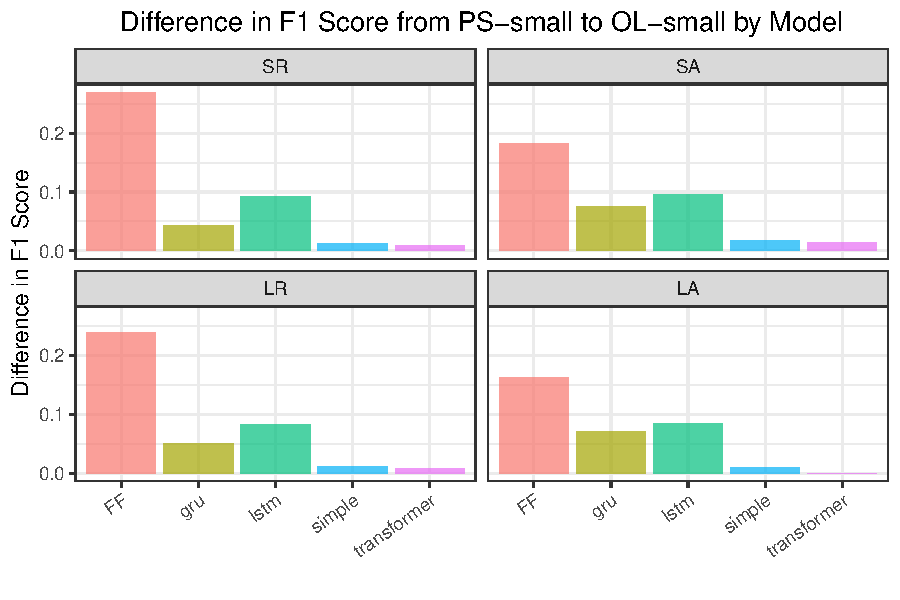
\includegraphics[width=\linewidth]{../analysis/figs/F1-diff-ps-ol-box.pdf}
\caption{Difference in F1 between \textsc{Small Plus Short} and \textsc{Only Short} by model \& test type.}
\vspace{-1em}
\label{fig:overall-diff}
\end{figure}

A third important observation is that there is a larger jump in
performance for the NNs from the \textsc{Small} to \textsc{Medium}
training conditions than there is for \textsc{FlexFringe}. From
\textsc{Small Plus Short} to \textsc{Medium Plus Short},
\textsc{FlexFringe}'s performance increases by about only 2 points,
whereas the NNs' performances increase about 5 points, except for the
LSTM which shows a nearly 15 point increase.

Taken together, these results suggest that \textsc{FlexFringe}
benefits far more from the inclusion of short strings, while the
neural models rely more on long strings to achieve their
performance. This seems to be particularly true for the GRU and LSTM
which see the large perfomance increases in the \textsc{Small} and
\textsc{Medium} conditions.

% Further breakdowns of performance by language class are given in
% Figures \ref{fig:os-by-class}-\ref{fig:ol-by-class} in the Appendix.

% \begin{figure}[t]
% \centering
% 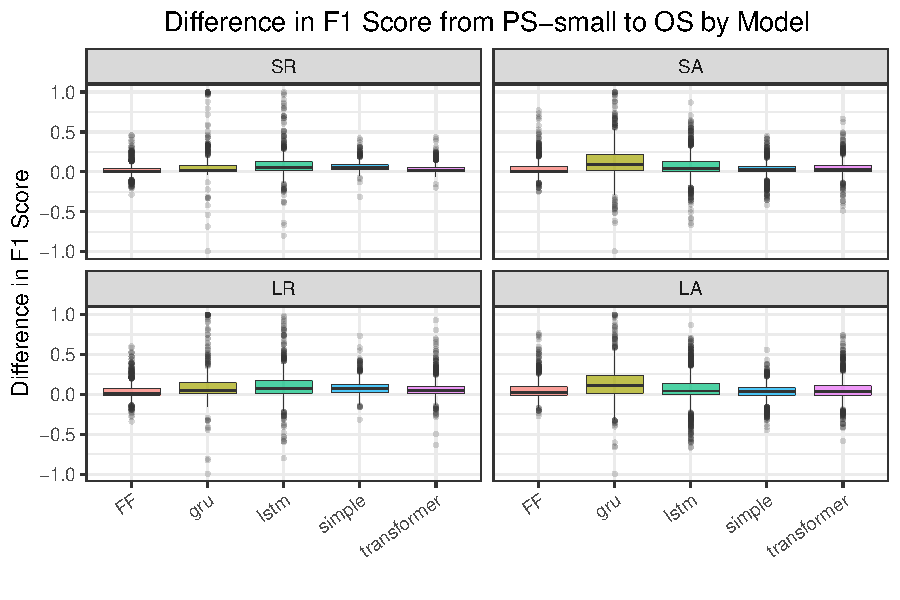
\includegraphics[width=0.8\linewidth]{../analysis/figs/F1-diff-ps-os.pdf}
% \caption{Difference in F1 between \textsc{PlusShort} (small training) and \textsc{OnlyShort} by model \& test type.}
% \label{fig:f1-diff-ps-os}
% \end{figure}

\subsection{FlexFringe Performance by Test Set}


% Friedman chi-sqaured is very significant 

% overall across all 5 conditions
%       LA        LR        SA        SR 
% 0.6407679 0.7141708 0.6618726 0.7405880 


% For each condition, it is also very significant; highest p-value = 8.724e-15

\begin{table}[t]
  \centering
  \begin{tabular}{lcccc}
  \toprule
    Training condition & SR        & LR        & SA        & LA        \\
    \midrule                                                
    Only Short         & 0.8223427 & 0.7690632 & 0.6998229 & 0.6585271 \\ 
    Small Plus Short   & 0.8412837 & 0.8074588 & 0.7388100 & 0.7125448 \\ 
    Medium Plus Short  & 0.8562071 & 0.8313988 & 0.7655567 & 0.7434051 \\ 
    Only Small         & 0.5698005 & 0.5607705 & 0.5315451 & 0.5240472 \\ 
    Only Medium        & 0.6133061 & 0.6021627 & 0.5736281 & 0.5653152 \\
    \bottomrule
\end{tabular}
\caption{Mean F1 scores by test type and training condition}
\end{table}

\subsection{FlexFringe Performance by Language Class}

%      coSL      coSP        LT       LTT       PLT        PT       Reg        SF        SL        SP     TcoSL       TLT      TLTT      TPLT 
% 0.7253188 0.5412781 0.6997698 0.7037642 0.7064781 0.6119616 0.7249771 0.7626772 0.7476214 0.6459687 0.6545515 0.6437818 0.6659095 0.6532684 
%       TSL        Zp 
% 0.6859998 0.8562712 


\subsection{FlexFringe Performance by Logical Level}


% 	Friedman rank sum test

% data:  data.matrix
% Friedman chi-squared = 12.4, df = 4, p-value = 0.01461

% > # POST HOC MULTIPLE COMPARISONS ANALYSIS
% > frdAllPairsNemenyiTest(data.matrix)

% 	Pairwise comparisons using Nemenyi-Wilcoxon-Wilcox all-pairs test for a two-way balanced complete block design

% data: y
%      CNL   DPL   FO    PROP 
% DPL  0.520 -     -     -    
% FO   0.992 0.797 -     -    
% PROP 0.899 0.100 0.665 -    
% REG  0.166 0.963 0.380 0.015


%      REG       DPL       CNL        FO      PROP 
% 0.7203313 0.7776397 0.7818242 0.7826672 0.7868925 


\subsection{FlexFringe Performance by }

% Friedman rank sum test

% data:  data.matrix
% Friedman chi-squared = 13.5, df = 3, p-value = 0.003671

% > # POST HOC MULTIPLE COMPARISONS ANALYSIS
% > frdAllPairsNemenyiTest(data.matrix)

% 	Pairwise comparisons using Nemenyi-Wilcoxon-Wilcox all-pairs test for a two-way balanced complete block design

% data: y
%       OTHER  PREC   SUCC  
% PREC  0.8443 -      -     
% SUCC  0.0655 0.0056 -     
% TSUCC 0.9472 0.9928 0.0138

% P value adjustment method: single-step
% > sort(colMeans(data.matrix))
%      PREC     TSUCC     OTHER      SUCC 
% 0.7555907 0.7768234 0.7768576 0.8064181 



\section{Conclusions}
The strongest model overall was the GRU, which performed best across
partitions.  Strikingly, however, the performance of the state merging
algorithm benefitted far more from the addition of short strings than
that of any of the neural models: it performed most competitively on
\textsc{OnlyShort}.  Meanwhile, increasing the size of the training
set was less helpful for the state merging algorithm than for the
neural models.  This shows a certain attunement of the state merging
algorithm to the kinds of input samples that are relevant for learning
natural languages \--- i.e., short and small.

Future research could expand the gridsearch (\S \ref{sec:ff}) to cover
additional parameters provided by \textsc{FlexFringe}.

\todo{future work}

\acks{Data set creation, model training, and evaluation were completed
  on the Stony Brook SeaWulf HPC cluster maintained by Research
  Computing and Cyberinfrastructure, and the Institute for Advanced
  Computational Science at Stony Brook University and made possible by
  NSF grant \#1531492. We also thank Sicco Verweer for his assistance
  with FlexFringe.}


% \section*{Code Availability}
% The code used for these experiments is available on \href{\repo}{GitHub}.\footnote{\href{\repo}{\repo}}.
% The code used for these experiments will be made available on GitHub upon publication.

\newpage
\appendix

\vskip 0.2in
\bibliography{refs}


\end{document}